\documentclass[conference]{IEEEtran}

\usepackage{graphicx}

\usepackage{placeins}

\graphicspath{{Figures/}}



\begin{document}

	\title{A Survey of Range-Only SLAM Techniques and Sensors}
	
	\author{\IEEEauthorblockN{David Grabowsky\IEEEauthorrefmark{1}, Samyak Shetty\IEEEauthorrefmark{2}, Sam Shue\IEEEauthorrefmark{3}, James M. Conrad}
		\IEEEauthorblockA{Department of Electrical and Computer Engineering\\
			University of North Carolina at Charlotte\\
			Charlotte, NC, USA\\
			\IEEEauthorrefmark{1}dgrabows@uncc.edu, \IEEEauthorrefmark{2}nshetty@uncc.edu, \IEEEauthorrefmark{3} slshue@uncc.edu, \IEEEauthorrefmark{4}jmconrad@uncc.edu}
	}
	
	
	
	\markboth{IEEE Transactions On xxxl, Vol. XX, No. Y, Month 2018}{Grabowsky: RO SLAM}
	
	
	
	
	
	
	
	\maketitle
	
	
	
	
	%The end of the abstract, I think, needs a better explanation of the survey other than stating that RO-SLAM techniques will be explored, ie: a more unifying theme
	\begin{abstract}		
		A common aspect in many autonomous robotics applications is addressing the problem of Simultaneous Localization and Mapping (SLAM). In most SLAM applications, the robot identifies distinguishable features in the environment, known as landmarks, through sensors such as cameras and laser rangefinders. Sensing these landmarks provide the robot with information such as range and bearing to the landmark, which are used in various algorithms responsible for determining the robot's pose and the landmark locations within the map. However, some applications have the restriction of using landmarks which are only capable of providing range information, such as wireless and acoustic beacons. Attempting to simultaneously localize and map with this restriction is termed Range-Only Simultaneous Localization and Mapping (RO-SLAM). This paper examines recent advances in the algorithms and technologies utilized to accomplish RO-SLAM.
		
		
		% In this survey, the variety of techniques used to solve the SLAM problem with respect to range only sensors is explored.
	\end{abstract}
	
	\section{Introduction} 
		%Possible way to breakup RO-SLAM methods other than by sensor type: indoor and out door
	
		The task of Simultaneous Localization and Mapping (SLAM) is a common aspect in many robotics applications. SLAM involves estimating the pose of a robot while simultaneously building a map of its environment with no priori knowledge of said environment. This task can be represented as a causality dilemma, where the pose of the robot is ascertained with respect to a global frame, or map, and the creation of a map requires knowledge of the robot's pose. There are a variety algorithms used to solve this problem, many of which use a landmark-based approach. Landmarks are distinguishable feature in an environment which can be observed via devices such as a camera or laser rangefinder. Said devices can be used to measure propeties such as the distance or bearing of the landmark relative to the robot. As the robot traverses the environment it continues to observe and collect landmarks while simultaneously building a map and localizing itself within the map. The sensed distance and bearing to each landmark can be combined with other factors like odometry readings to get an refined estimation of the robot pose and map. 
		%It can continue observing that landmark, as well as collecting new landmarks, and using the sensed distances and angles combined with odometry readings to refine its estimation of the robot's pose and map. 
	%	In most SLAM applications, references to the map is synonymous with the locations and features of the landmarks.
		

		%Ohhhh my good  this feels so jaring to read. I don't think odometry was ever properly introduced either
		In outdoor SLAM applications, such as self-driving cars and autonomous farming equipment, global positioning satellite (GPS) measurements are used to help localize a vehicle. %ADD A CITATION
		While GPS has low resolution, it proves useful as it provides location information, which can help compensate for the accumulated error from drift in odometric sensors. However, GPS isn't available in all environments, such as indoors and underwater. Instead, wireless signals and sonar beacons are often are utilized. These beacons provide range data, but do not inherently provide location information as with GPS. However, these distances are often still useful as they can be used to compensate for the drift that occurs from measuring a vehicle's displacement through integration of inertial sensor readings. Most SLAM algorithms utilize these range values as a corrective measurement, the same way traditional algorithms use sensed landmarks. However, rather than using range and orientation to landmarks, beacons are only capable of providing range. SLAM algorithms which utilize these beacons are referred to as Range-Only SLAM (RO-SLAM). 
		
		While the loss of orientation from traditional, vision based landmarks  proves to be a detriment, range only beacons solve two major problems encountered in traditional landmark-based approaches: landmark association and landmark scaling. The landmark association problem occurs when a detected landmark has similar features to previously recorded landmark and is mistaken for the other, generating huge errors in the estimation of both the robot and the landmark. This problem is avoided using beacons, as they have some kind of network address which is broadcast during transmissions, so there is no way to confuse which range is associated with which landmark. The scaling problem occurs when a SLAM algorithm runs for a long time and more and more landmarks are appended to the map. As more landmarks are added, the amount of memory needed to store the positions and distributions of these landmarks increases, as well as computation time. When using beacons, a finite number of landmarks exists, and the total size of the map is known before deployment. In addition, fewer landmarks are needed in beacon-based applications, as most beacons do not require line-of-sight to be measured, unlike visual landmarks. Since the robot can observe the landmarks more often, it doesn't need to add nearly as many to ensure accurate position estimation. %Need a citatation to back that claim up
		
		%Eh... probably some better phrasing for this paragraph
		This paper surveys state of the art RO-SLAM applications. Before discussing RO-SLAM techniques, the different types of range sensors are introduced in Section \ref{range only sensors}, followed by initialization of range beacons in Section \ref{beacon initialization}. Solutions to the RO-SLAM state estimation problem are covered in Section \ref{methods and their implementations}. Finally, the conclusion in Section \ref{conclusion} closes with final thoughts regarding the state of the field of RO-SLAM.
	
	
	\section{range only sensors}
	\label{range only sensors}
		There are a variety of sensors which can be utilized as range-only beacons for RO-SLAM. These range sensors refer to any device which involves a signal transmission that can be used for the range estimation without requiring line of sight. The most popular sensors can largely be broken down into two categories: acoustic based and radio frequency based. These two types of sensors both largely rely on the same principles for measuring distances, which are either signal time of flight, or signal attenuation through propagation through each respective medium. These beacons serve as the landmarks within the RO-SLAM algorithms map and can have a significant impact how the algorithms are implemented.
	
		%I think this section could use some more details. 
		
		%HOLY moly does acostic sensors need mor details
		\subsection{Acoustic}
	
			Acoustic ranging systems are largely used with autonomous underwater vehicles (AUV) that operate in underwater locations. The reason for this is that radio waves experience strong attenuations in salt water environments. As Partan states, the issue of attenuation makes radio waves extremely impractical, thus making acoustics the logical alternative \cite{Partan2007}. Acoustics still suffer from a range of problems such as multipathing and propagation delays, but compared to the alternatives they perform adequately in underwater environments. For those seeking additional information about the constraints imposed by underwater environments on acoustic sensors see \cite{Erol-Kantarci2011} and \cite{Akyildiz2005}. These papers explore a wide variety of issues and possible solutions that relate to acoustic sensors, such as the added complexity of assuming a two dimensional versus a three dimensional environment, or the design challenges that accompany underwater deployment with regards to spatial correlation and power consumption. 
		  	
		  	
		  	%Ehhhhh.. This section... I dunno if this section is necissary
			A unique implementation of an underwater acoustic beacons is the Dive'N'Rise (DNR) beacon presented by \cite{Erol2007}. These DNR beacons rise to the surface, receive their location through GPS, then sink into the water and transmit their coordinates. The distance between an robot and the transmitting beacon can be determined via time of flight from the transmissions and used in conjunction with the GPS location to determine a refined location for the beacon. A localization implementation using these beacons was accomplished by \cite{Erol2008}. 
	

		\subsection{Radio Frequency}
			
			This subsection encompasses an extensive spectrum of devices capable of transmitting or receiving signals using radio frequencies (RF). There are two methods commonly utilized to determine distance from radio frequency. One is by examining the received signal strength indicator (RSSI) and the other is by measuring the time of flight of the signal. A system presented by \cite{Padmanabhan2000} processes RF signal strength and utilizes nearest neighbors heuristics to achieve localization based on said signal strength.  \cite{Kurth2003a} describes a method for using very small RF tags as beacons in an environment.  As a mobile robot moves throughout the environment it emits a query to which any RF tags that are within the transmission range respond. The robot then estimates the distance to the tag based on the delay. The response from the RF tags include a data tag which contains a unique ID number. 
						
			Wireless Fidelity (wi-fi)  is the a popular beacon choice as existing networks are already prevalent in many indoor locations and they are generally low cost \cite{Youssef2005} \cite{Sen2013} \cite{Kotaru2015} \cite{Rea2017}. \cite{Youssef2005} presents a system known as Horus with the aim of high accuracy and low computation cost for wireless local area network location determination. \cite{Sen2013} proposes a method named CUPID which extracts information from the physical layer to process information allowing it to avoid the impact of multipathing. \cite{Kotaru2015} presents a design and implementation for its SpotFi system which can be deployed on top of existing wi-fi infrastructure. \cite{Rea2017} designed a new method for filtering range measurment specifically designed with the large noise found in indoor WiFi radios in mind. 

			 Another popular wireless standard often used in wireless ranging and localization applications is IEEE 802.15.4, which has been largely popularized by the ZigBee protocol. In contrast with IEEE 802.11 WiFi standards, 802.15.4 is focused on shorter-ranged, low power peer-to-peer networks, thus making it a widely used protocol in Wireless Sensor Networks (WSN).  \cite{Baronti2007}, \cite{Khanafer2014},\cite{Shue2013}, \cite{Akyildiz2002}, and \cite{Xia2011} each present surveys relating to WSNs. \cite{Baronti2007} and \cite{Akyildiz2002} both provide very well developed surveys that discuss hardware, protocols, standards, security, energy efficiency and much more. \cite{Baronti2007} specifically focuses on wireless sensors utilizing ZigBee standards. \cite{Xia2011} examines the limitations of original IEEE 802.15.4 MAC and reviews adaptive methods that have been used to overcome these limitations. \cite{Khanafer2014} specifically survey methods meant to improve the performance of IEEE 802.15.4 MAC protocol. \cite{Shue2013} surveys the application of robotics in wireless sensors by examining topics such as data mules, sensor failures, and node localization. 
			 
			 Ultra-wideband (UWB) radios are another popular choice. One attractive feature of currently used ultra-wide band transmitters and receivers is the ability resolve multipath error ,which is a common obstacle with indoor environments, without the use of extensive algorithms due to its use of multiple frequencies across a large bandwidth. \cite{Gezici2005} presents an analysis of time of arrival based localization estimations with ultra-wide band. 

			%blue tooth
			
			
			%wifi
			
			%Fingerprint map based on radiological patterns
			%P. Bahl and V. Padmanabhan, “Radar: A, in-building rf-based user
			%location and tracking system,” in Proc. of the IEEE Infocom, 2000,
			%pp. 775–784.
			
			%M. Oca ̃na, L. M. Bergasa, M. A. Sotelo, R. F. Flores, D. F.  ́
			%Llorca, and D. Schleicher, “Automatic training method applied to
			% WiFi+ultrasound POMDP navigation system,” Robotica, vol. 27,
			%no. 07, pp. 1049–1061, December 2009.
			
			
			%rfid
			%Mapping and localization with RFID technology

	\section{Beacon Initialization}
		\label{beacon initialization}
		The core motivation of SLAM algorithms is the exclusion of a priori knowledge of the operating environment. This includes locations of landmarks. Because of this, landmarks are appended to the map as they are discovered in traditional SLAM algorithms, using the robot's estimated pose and the sensed distance and orientation to estimate an initial position of the landmark. The landmark's positions is then refined as the algorithm continues to run.
		
		The same process occurs in RO-SLAM, however, the landmark's initial position is not so easily determined, as the range-only beacon has an unknown orientation relative to the robot. Therefore, the landmark could reside approximately anywhere within the sensed distance radius. To compensate for this, most beacons go through an initialization phase before being appended to the map and utilized in the RO-SLAM algorithm. This initialization phase is usually performed over several iterations until the position converges to an acceptable degree.
		
		One RO-SLAM complication in particular involves the issue of EKF-SLAM, which is used by many implementations, being  sensitive to poorly initialized landmarks as they are used as the basis for the convergence of an accurate estimate. Poorly approximated landmarks results in the divergence of the filter. 
		
		Presented here are the most effective and commonly used methods to initialize range beacons. These methods are further divided into delayed and undelayed initializations.
		
		\subsection{Delayed/Offline initializations}
			Delayed/offline initializations are methods which attempt to localize the beacon prior to incorporating it into the active SLAM algorithm. Some SLAM algorithms require an approximate location of each landmark before being incorporated into the algorithm. Since beacons only provide range data, the location of the beacon is not known upon first observation, and must be initialized. These processes which determine the initial estimated location of the beacon before being added to the SLAM algorithm are known as delayed or offline initializations. These initialization methods can be undesirable as they require the SLAM algorithm to run without corrective measurements until the first beacon is initialized. Presented in this section are the most prevalent methods for offline beacon initialization.
			 
			\begin{figure}
				\centering
				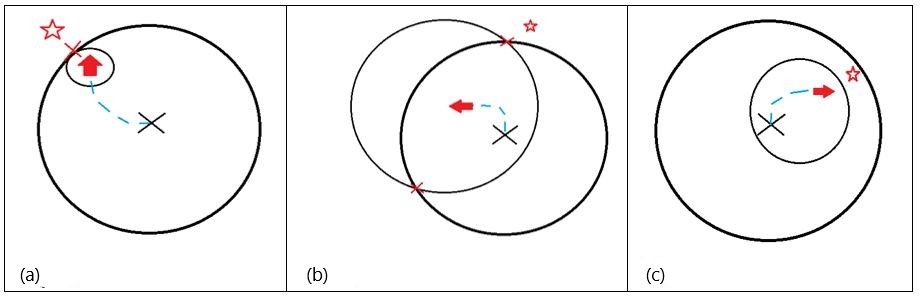
\includegraphics[height=30mm,width=90mm]{Trilateration_methods.JPG}
				\caption{The red arrow represents the robot.The 'X' represents the origin of the robot. The blue line shows the traversed path.The star represents the landmark. }
			\end{figure}
		
			\subsubsection{Trilateration}
				Trilateration refers to the process of using the distance to at least three devices at known locations in order to estimate the location of a fourth device. Methods generally utilize the geometry of circles and triangles in order to accomplish this \cite{Johnson2017}. \cite{Thrun2002} mentions a basic trilateration technique involving geometric intersection. Rings are drawn at different points of the robots path as shown in Fig[a], where the radius of the rings depend on the strength of the received signals from the beacons. This method of initialization is highly ambiguous as the rings can have more than 1 point of intersecting as shown in Fig[b]  or no  intersecting points as shown in Fig[c]. %more papers needed
		
			\subsubsection{Particle filter}
				The particle filter takes a probabilistic approach to estimating the initial location of the beacons as mentioned in \cite{Thrun2002a}. Here, a particle refers to a  possible hypothesis of position of the beacon/landmark. 
				
				Initially the robot assumes global uncertainty through a set of particles that are uniformly distributed over the map as shown in Fig 2.(a). Hence the position of the beacons are uncertain. As the robot moves around and measures sensor data it re-samples the particle set based on computed weights. Particles that match sensor data are assigned higher probabilistic weights and are therefore more likely to be re-sampled each iteration. Fig.2(b) illustrates this, as particles with hypothesized beacon locations far from the true location do not match the sensed range and over time are eliminated from the set. After many iterations only the particles which have a high degree of probability  remain and eventually converge to the true location of the beacons as shown in Fig.2(c). There are several re-sampling methods which are discussed in \cite{Li2015}.
				\begin{figure}[h!]
					\centering
					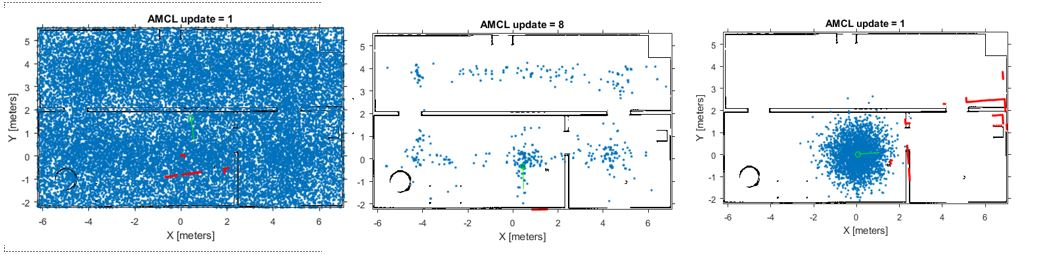
\includegraphics[height=35mm,width=90mm]{Particle_filter_method.JPG}
					\caption{The leftmost image describes the state of the robot when it just initializes the particle filter. The particles are uniformly distributed. The image in the center describes the particle filter after a couple of iterations. Only the particles which have a higher probability are re sampled. The image on the right shows the particle filter eventually converging to estimate the beacon location. }
					
				\end{figure}
				Assuming at time t=0;we have N particles equally space in the environment that are drawn based on a uniform distribution $ p(x_oa)$.                                                                       
				Once the robot starts moving it collects measurements and at time $t>0$ we sample a new particle set $x^{[i]}_t$ for each particle in $x^{[i]}_{(t-1)}$. It is sampled based on the probability of measurement $p(z_t|x^{[i]}_{(t-1)})$. Eventually the particle filter converges to give us the true positioning of the beacons.
				 These particles are re-sampled based on importance weights every iteration. There are several re-sampling methods mentioned in \cite{Li2015}. Eventually the particle set converges to the accurate location of the beacons. 
				
			\subsubsection{Other Methods}
			 	The methods presented above tend to be the more common approaches, however, there are several offline algorithms that perform offline localization. A least squares approach is described in \cite{Newman}, a posed-based EKF (Extended Kalman Filter) method is mentioned in \cite{Webster2012}, and a moving horizon estimation is presented in \cite{Vallicrosa2014a}. These methods have also proven effective for the beacon types used in their respective applications.
			

		\subsection{Undelayed/Online initializations}
			With undelayed/online initializations simultaneously initializes and localizes itself and the beacons as it moves, as mentioned in \cite{Caballero2010}. A Gaussian Mixture Model is integrated into the EKF to create a multiple hypothesis filter.  This multiple hypothesis approach is used to solve the RO-SLAM problem and its use allows for the un-delayed initialization of landmarks, however a large number of hypothesis can lead to increased computational burden. \cite{Geneve2015} presents a method that models a Gaussian mixtures for beacon initialization in EKF. This method only uses two hypotheses and a Cartesian plane. \cite{Ahmad2011a} proposes to reduce the computational burden of methods, such as the one proposed by \cite{Caballero2010}, by introducing a novel state vector that eliminates the need for multiple hypothesis landmark representation. The paper proposes that under different circumstances the landmark could be represented using different parameters. This representation would lead to reduced computation cost for large scale range only SLAM as opposed to the high computation cost of multiple hypothesis landmark representations. Four circumstances are presented in the paper and the method is tested in simulation using both the EKF and a least squares optimization approach. The results showed that when the circumstances can be clearly distinguished between, an increase in performance is seen.



	
	

	\section{Methods and Their Implementations}
	\label{methods and their implementations}
	The following implementations are broken down into categories based on the general algorithm that is used by the implementation to do RO-SLAM. The concept behind the algorithm is summarized in each category followed by a discussion of implementations that incorporates said algorithm. Each category concludes by examining the problems that current implementations are focusing on and theorizing about possible future directions for research.  
	\subsection{EKF}
	
	%breif description (1-2 paragraphs)
	
	%paragraphs 
	
	The Extended Kalman Filter (EKF) is one of the most popular and widespread methods used to solve the SLAM problem. It is used to overcome the assumption of linear state transitions and measurements, which are rarely seen in practical environments \cite{Thrun2002}. The derivation of the EKF is very well documented, as such, detailed explanations can be viewed from a variety of sources such as: \cite{Thrun2002}, \cite{Ribeiro2004}, and \cite{Haykin2001}. Generally, EKF can be broken up into two phases, the prediction and the measurement phase. The prediction phase updates the state vector based on control inputs and additive Gaussian noise. The measurement phase updates the state vector based observed landmarks with additive Gaussian noise.
	
	 When used to solve SLAM the map applied to the EKF is a feature based map, meaning it is composed of observable features (landmarks) which can be distinguished between during re-observation \cite{Thrun2002}. This distinction becomes important when examining RO-SLAM where only the range to a landmark, or the range between landmarks, is known. 
	 %This restriction means that landmarks often need to be manufactured 
	 %add rererence here...
	 %, such as the beacons discussed in previous sections, and physically placed in an environment. 
	 In addition, the exact location of the landmarks, or even there initial existence, is not always known at the beginning of runtime. Initialization is a critical element in many algorithms that make use of the EKF. If the initialization is inaccurate then the convergence to a correct estimation can become much more difficult. The EKF has seen a wide variety of implementation ranging from ground based robotics\cite{Djugash2008} \cite{Shue2017}, to unmanned air vehicles \cite{Fabresse2016}, and to autonomous underwater vehicles \cite{Olson2006}. This section will proceed to give a summary of the various ways EKF has been implemented in regards to RO-SLAM.
	
	%Underwater implementations
	A system for robust range only localization was prosed by \cite{Olson2006}. The system utilized an Autonomous Underwater Vehicle (AUV) and beacons without carefully surveyed locations. The paper notes that one of the majors issue was noise present in the received data. A method for outliers rejection caused by the noise was accomplished via spectral graph partitioning. A voting scheme was implemented similar to a Hugh transform to get approximate beacon locations \cite{Hough1959}. The approximate locations were then incorporated into an EKF. It is noted by the paper that this method is particularly CPU intensive, however they state that since the rate at which data is acquired from a landmark is slow, every 5 or so seconds, that the AUV can afford the expensive computation since there will be an adequate amount of time between readings for the data to process. The methodology was simulated using a dataset and can be seen in the paper.
	
	
	%AUV implementations
	\cite{Kurth2003} presents a comparison of how three methods process a collected data set. The methods are a EKF, a sliding batch, and a particle filter. The comparison considers the cross-track error, and along track error. The results state that the particle filter works well when used to acquire an initial pose estimate, and EKF works well with real-time localization. It is suggested that in the future that the two could be switched between when appropriate to improve the overall system. 
	
	
	
	
	
	
	
	%fabreese. 
	
	%1. 2013 presents EKF slam method for ariel vehicles 
	
	%2. 2014 introduces prefiltering to measurments for previous 
	
	%3. 2014a integrates visual landmakrs as well
	
	%4  2015 decentralized multiple arieal vehicles
	
	%5  2016 specifically unmaned ariel, more details on 2013,2014 and experimental validation of 2013,2014.
	
	
	
	\cite{Vallicrosa2015} presents a solution utilizing a Sum of Gaussian (SOG) filter for a single range only beacon. It uses multivariate Gaussian mixtures to represent the probability distribution functions of the robot and beacon positions as Gaussian particles which each contain an EKF for vehicle position, velocity, and estimated beacon position. The paper presented experimentation where the method was used to map a beacon while correcting the navigation of the vehicle. 
	
	
	
	Several techniques have also been implemented that involve cooperative sensors. Traditionally sensors were used to only determine the range between themselves and the robot. The sensors in these cases provide the ability determine the range between themselves and other sensors and or the robot \cite{Patwari2005}.
	
	\begin{figure}[h!]
		
		\centering
		
		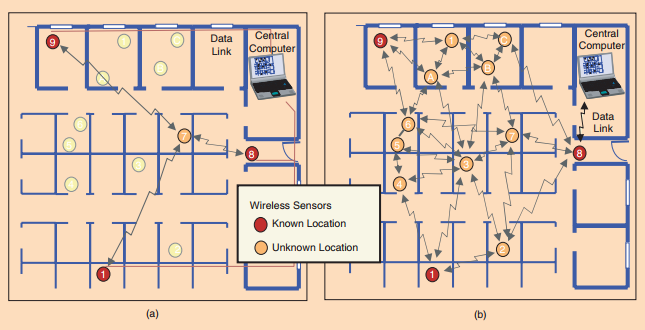
\includegraphics[width=90mm]{coop_loc_comp_patwari.png}
		
		\caption{Traditional(a) vs Cooperative(b) Sensors \cite{Patwari2005}}
		
		\label{trad_vs_coop_sensors}
		
	\end{figure}
	
	\FloatBarrier
	
	
	
	It is explained by \cite{Torres-Gonzalez2015} that methods utilizing inter beacon measurements should incorporate measurements with a configurable number of hops between beacons. This allows for the robot to gather range data from beyond the extent of the robots sensors. Experimentations was conducted utilizing this method via a particle filter EKF. The results showed that the more hops that were added the greater the performance of the system. 
	
	
	
	\cite{Djugash2006} presents a comparison of multiple RO-SLAM methods utilized in two scenarios. One scenario involves the case where the robot only has access to range information between itself and beacons at unknown locations. In the second case the robot also has access to information about beacon to beacon distances. Several separate methods were compared in the given scenarios utilizing a data set and experimentation. The first method utilizes the Kalman filter in the case where only measurement between moving and stationary beacons are considered. Another method specifically uses the beacon to beacon measurements with an online Kalman filter. An off line batch method is used to get an estimate of the beacon location and robot path. Finally an method that considers the robot as a virtual node for creating submaps to be solved with a multidimensional scaling algorithm is also considered. The paper gives experimental results and analysis for each of the methods. 
	
	
	
	%In scenarios where the location of the landmarks is unknown and each landmark can not communicate with all every other landmarks, \cite{Djugash2006} presents a solution. He proposes that a moving beacon be used to add edges to the network \cite{Djugash2006}. In addition, no external position sensing were required on the part of the moving beacon, but the option for it to be incorporated was available. 
	
	
	
	
	
	
	An extension to EKF called relative-over parametrized (ROP) EKF is presented by \cite{Djugash2008}. This extension uses specific parameterization to  better represent the range only data utilized in RO-SLAM. ROP EKF operates in polar coordinates as opposed to the Cartesian space that typical EKF operates. The method provided improved results over EKF when sparse range measurement or data association errors were present. \cite{Herranz2014} presents a comparison of the ROP-EKF method presented by \cite{Djugash2008}, to a smoothing and mapping method presented by \cite{Dellaert2006}. Experimentation conducted by \cite{Herranz2014} on and indoor and outdoor environment show an improvement in the results of the smoothing and mapping (SAM) method over ROP EKF.
	
	\begin{figure}[h!]
		
		\centering
		
		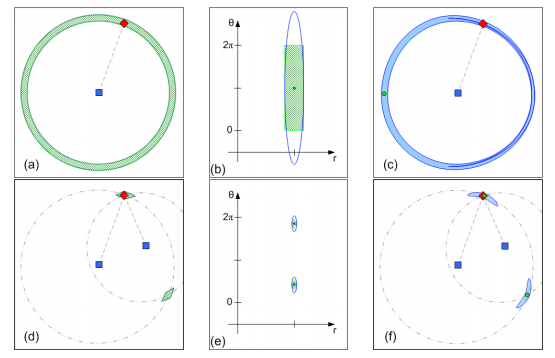
\includegraphics[width=90mm]{ROP_djugash.png}
		
		\caption{Top Row: True and approximated distribution from one range observation. Bottom Row: True and approximated distributions with two observations from different locations. Left Column: Distribution in Cartesian Coordinates. Middle Column: True and Gaussian approximated distributions in Polar Coordinates, Right Column: Projection of the Gaussian approximated. \cite{Djugash2008}} 
		
		\label{ROP_djugash}
		
	\end{figure}
	

	
	
	A method proposed by \cite{Dios2015} is geared towards improving map building speed and accuracy for unmanned aerial systems dealing with the 3D RO-SLAM problem. The 3D RO-SLAM problem refers to the added complexity that devices such as submersibles \cite{Newman} and aerial vehicles experience when having to operate in an environment where three dimensions must be considered as opposed to the planar environment many robots are assumed to operate in. The method utilizes inter-beacon measurements and a novel mode selection which is used to select a measurement gathering method based on current conditions \cite{Dios2015}. The first mode is noted as mapping (MS) and the second localization (LS). When in mapping mode the measurement are integrated with a high probability to quickly create a map, when in localization mode the probability is lowered to create higher accuracy localizations. Based on experimentation performed by \cite{Dios2015} the method performed well and a general increase in accuracy and map speed was noted, however it is stated that a wider variety of experimentation should be performed to validate the overall robustness and effectiveness of the method.
	
	%this one might need some more work
	
	
	
	\cite{Kehagias2006} explores how interpolation can be used to generate range data that is equally spaced over time as opposed to the irregular time intervals that range data is typically received at and then applied to solve the RO SLAM problem. The method is tested on the EKF and an batch optimization algorithm with a simulated and physical robot. The results provided by the paper show that the interpolation based algorithms gave better landmark estimation than those without, with the exception of the EKF in two datasets where EKF was already performing poorly.
	
	
	
	
	
	\cite{Fabresse2013} presents a solution for the 3D RO-SLAM problem. The solution reduces computational load through reduced spherical parametrization of map feature positions. The paper also proposes a new EKF update method which incorporates a reduced spherical representation of the state vector. In addition the paper describes how to efficiently integrate multi-modal belief of elevations angles and azimuth from a range sensor into the EKF utilizing two independent Gaussian Mixtures \cite{Fabresse2013}. In addition \cite{Fabresse2014} expands upon this by presenting a pre-filtering algorithm to be applied to range measurement before being used in the EKF in order to reduce the effect of noise generated by environmental issue such as multipath. It is then proposed by \cite{Fabresse2015} that the above method can be utilized for decentralized multi-SLAM with range only sensors. This new method would allow for landmarks estimated by a robot to be incorporated into the estimation of another nearby robot, thus improving localization estimation. Based on experimental results obtained by \cite{Fabresse2015} the integration of estimates from multiple robots of the same landmarks provides a benefit to landmark localization over a single robot. In \cite{Fabresse2016} the author also validates and expands upon this method through indoor and outdoor experimentation with an Unmanned Aircraft System (UAS).  
	
	
	A common focus of many recent papers has been the utilization of beacons for more than just robot to beacon range measurements. Such implementations now use beacons to perform tasks such as measuring ranges to other beacons in addition to the robot. These beacon to beacon range measurements are then incorporated into existing EKF algorithms. Beacons are also utilized to off-load certain processing.
	
\subsection{Sparse Extended Information Filters}

Information filters work on the same underlying Gaussian belief principle as that of EKF but vary in the way that Gaussian beliefs are represented. An information filter (IF) algorithm is mentioned in\cite{Torres-Gonzalez2014}. In EKF the Gaussians are represented in the form of their moments, mean and variance, whereas in a information filter the Gaussians are in their conical parameterization which comprises of an information matrix and information vector. 
%Hence what is computationally complex in EKF is simple in the other and vice versa. Hence they are dual to each other.
Sparse Extended information filters are derived from the  information filter but it maintains a sparse representation of the information matrix. This makes the SEIF more scalable and efficient as show in \cite{Torres-Gonzalez2014}.

%Jeez, this explains the information filter in suuuuch abstract terms
The information filter stores the relation between any two state elements in the information matrix also known as links. The higher the value of a link, the stronger the relationship between two state variables which in turn affects the robots state. SEIF maintains a sparse information matrix by eliminating weak links that are below a certain threshold thus reducing the computational complexity involved.

In \cite{Torres-Gonzalez2014} the computational complexity is reduced by utilizing the computational capabilities of the nodes or radio  beacons. Here the robot computes the prediction stage of the iteration, sends the information to the beacons where the update process is completed. Hence the computation burden on the robot is reduced. In addition, inter-beacon measurements are factored in to reduce uncertainty even further. In \cite{Torres-Gonzalez2017} the SEIF method is evaluated and compared for 3d SLAM using an octorotor In conclusion this method had better estimates and lesser computational burden than the traditional RO SLAM method using EKF. \cite{Torres-Gonzalez2017a} extends this method by integrating a distributed information-driven measurement allocation tool with the SEIF to allow for dynamic selection of measurements. The end goal being to create a scheme that utilizes robot-beacon and inter-beacon measurements to increase accuracy while maintaining resource-consumption efficiency and scalability. Thus, creating a scalable distributed RO-SLAM scheme with a focus towards resource limited operations.



	
	
	

	
\subsection{Particle Filters}      %change the references
Particles filters are a category of monte carlo algorithms. They are used to estimate states in partially observable Markov chains as shown in \cite{Doucet2001}. In  early applications, particle filters were used in the field of localization where it was used to estimate a robots pose from sensor data. It is considered better and more robust to conventional estimation methods because of its ability to solve the global localization \cite{Borenstein1996} and the kidnapped robot problem \cite{Engelson1992} which EKF, in comparison, struggles with. At is core, EKF also has higher dimensional computation problems.
% It has also been at the core higher dimensional computational problems.  
%Description
As mentioned in \cite{Thrun2002a}, particle filters outperform EKF in applications involving global localization (the kidnapped robot problem) where the robot is randomly picked up and placed in a unknown environment. 
EKF cannot process negative information, but since particle filters use raw sensor data without any processing they can process negative information\cite{Thrun2002a}. 

It works in a similar way to the particle filter initialization procedure mentioned in Section \ref{beacon initialization}, but it uses a weighted average of both the possible landmark and robot positions to converge to the actual robot and landmark locations.

As the number of particles increases the computational complexity of the filter too increases. In order to address this there were several new methods introduced that  exploit the independence among state variables. For example the Rao-Blackwellized particle filters that exploit the independence of the landmarks with the robot path thereby reducing the computation complexity from \cite{Yuan2012}. It also solves the data association problem previously unsolved by EKF. Although this method of localization can be computationally expensive it is preferred whenever the noise involved is non Gaussian.
	

   \cite{Blanco2008a} uses the particle filter to overcome the delayed initialization issue brought forward by RO SLAM. It uses the Rao-Blackwellized Particle filter to maintain a conditional distribution for each beacon which eventually is transformed into a EKF when the uncertainty becomes sufficiently small. This approach is validated for both simulated and real data sets. This approach is preferred in indoor applications where there is a high probability of multi path signal propagation.

	
	
	
	%Brief introduction
	
	
	
	
	
	
	
	%advantages
	
	%Disadvantages
	
	
	
	
	
	\section{Conclusion}
	\label{conclusion}
	This paper has introduced the motivation and practicality of RO-SLAM approaches. The variety of sensors used as range only beacons has been surveyed, along with initialization methods for their incorporation into the common SLAM algorithms. The variety of SLAM algorithms as they apply to range-only sensor data are surveyed here as well with a focus on the techniques that differentiate them and highlighting their strengths and weaknesses.

	Given the maturity of SLAM as a research field, the area of RO-SLAM still has lots of area to explore. Most of the common methodologies presented here focus on adapting traditional SLAM algorithms to accommodate only range data. While these adapted methods have been proven successful, there is still more research that can be conducted towards solving the RO-SLAM problem with uniques solutions which can subvert the need for offline beacon initialization and models designed to handle the multipath errors which plague range sensors.
	
	
	
	
	\bibliographystyle{IEEEtran}
	
	\bibliography{references}
	
	
	
\end{document}